\subsection{Vergleich von CAD-Viewer Programmen}
\label{subsec:comparison-cad-viewer}

Wir wollen die nachfolgend aufgelisteten, kostenlos verfügbaren, CAD-Viewer Programme testen.
Die Produkte sind durch eine Internetrecherche zum Thema CAD-Viewer aufgetaucht.

\begin{enumerate}
    \item Autodesk Viewer
    \item DWG TrueView
    \item eDrawings Viewer
    \item ABViewer
    \item DWG FastView
\end{enumerate}

Danach sollte eine Auflistung von Anforderungen möglich sein, die - neben den bereits gegebenen Anforderungen - für das neue Visualisierungswerkzeug für Gebäudepläne sinnvoll erscheinen.

\subsubsection{Autodesk Viewer}
\label{subsubsec:autodesk-viewer}

Das Programm \textit{Autodesk Viewer} vom ursprünglichen Entwickler des DXF-Formats Autodesk~\cite{DXFReference} ist eine web-basierte Lösung zur Ansicht von CAD-Dateien~\cite{AutodeskViewer}.
Zur Verwendung reicht ein Browser und ein Aufruf von https://viewer.autodesk.com sowie ein vorhandenes Benutzerkonto bei Autodesk.
Ein Screenshot davon ist in Abbildung~\ref{fig:autodesk-viewer} zu sehen.

Die Dateien zur Ansicht müssen dort hochgeladen werden.
Danach kann im Beispielgebäudeplan per Maus navigiert werden (Mausrad zum Anpassen des Maßstabs, Ziehen mit der Maus zum Verschieben).
Des Weiteren stehen Funktionen zum Messen zwischen verschiedenen Punkten und zum Markieren einer bestimmten Stelle oder eines Bereichs zur Verfügung.
Außerdem kann der Anwender den geöffneten Gebäudeplan im Rastergrafikformat PNG herunterladen.
In der resultierenden PNG-Dateien befinden sich auch alle vorgenommenen Markierungen und Messungen.

\begin{figure}
    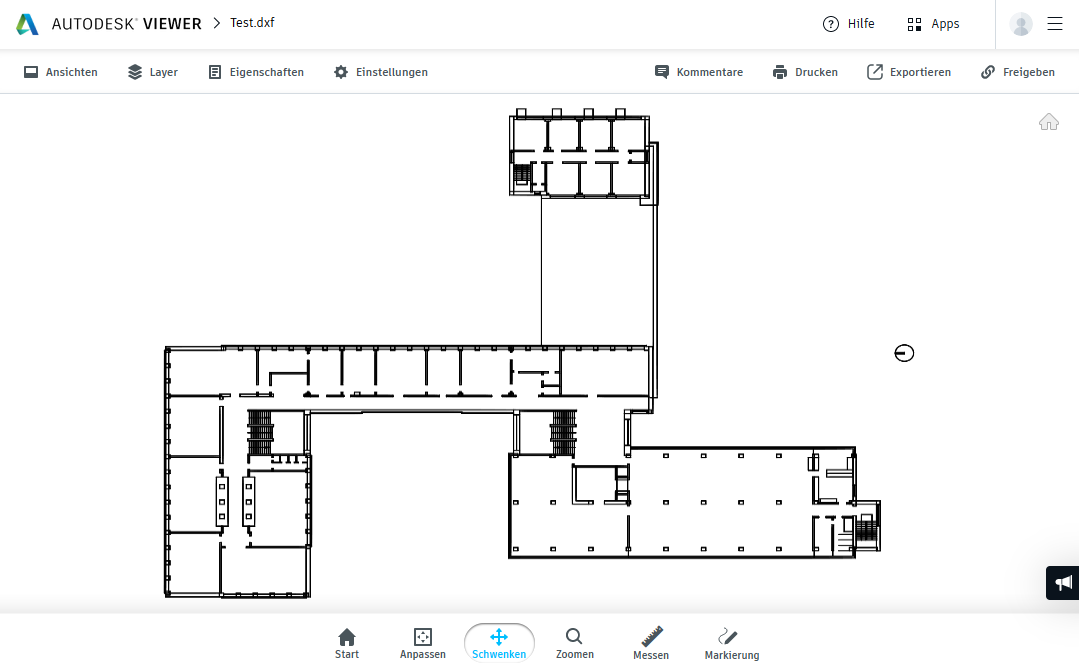
\includegraphics[width=0.5\textwidth]{res/autodesk-viewer.png}
    \caption{Screenshot des Programms \textit{Autodesk Viewer}.}
    \label{fig:autodesk-viewer}
\end{figure}

\subsubsection{DWG TrueView}
\label{subsubsec:dwg-trueview}

\textit{DWG TrueView} ist wie Autodesk Viewer ein Produkt vom Hersteller Autodesk~\cite{DWGTrueView}.
Im Gegensatz zu Autodesk Viewer ist jedoch eine Installation des Programmes notwendig, dessen Setup-Programm aktuell eine Dateigröße von über einem halben Gigabyte aufweist.
Zur Installation sind derzeit weitere 1,42 Gigabyte notwendig.
Nach dem Laden unserer Beispieldatei sieht das Programm wie in Darstellung~\ref{fig:dwg-trueview} abgebildet aus.
Laut einer Vergleichsseite von Autodesks Viewerprogrammen unter https://www.autodesk.de/viewers/all-viewers/compare unterscheidet sich das Programm von Autodesk Viewer nur unwesentlich und unterstützt weniger Dateiformate.

Vom Featureumfang unterscheidet es sich zu Autodesk Viewer lediglich durch eine Option zwischen verschiedenen DWG Versionen zu konvertieren (Autodesks proprietäres CAD-Dateiformat~\cite{DWGTrueView}).

\begin{figure}
    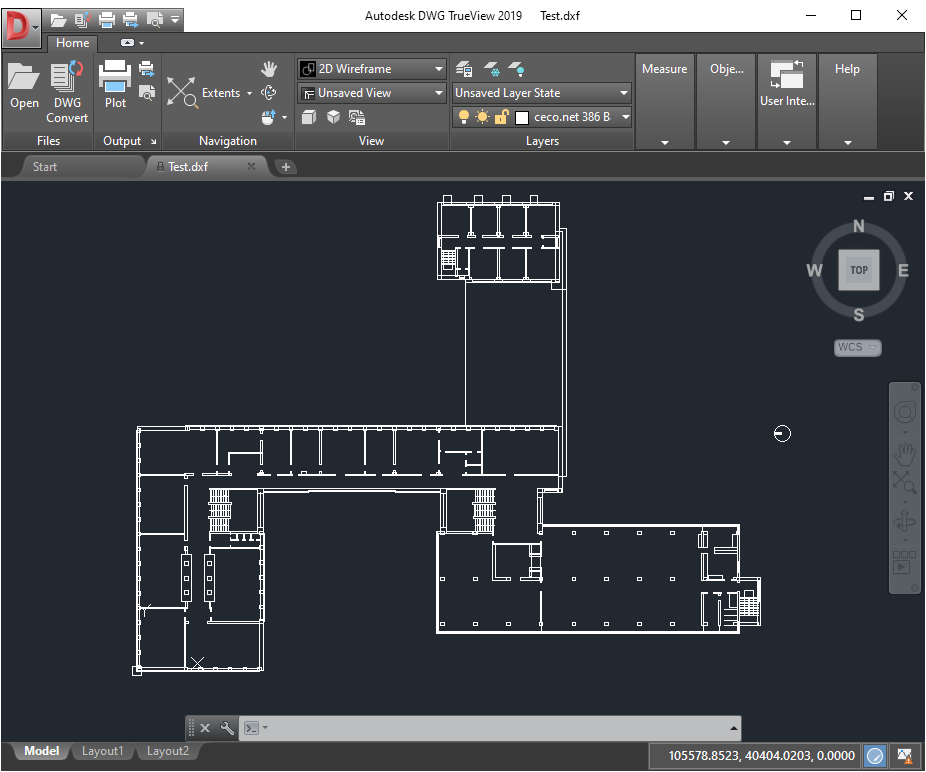
\includegraphics[width=0.5\textwidth]{res/dwg-trueviewer.png}
    \caption{Screenshot des Programms \textit{DWG TrueView}.}
    \label{fig:dwg-trueview}
\end{figure}

\subsubsection{eDrawings Viewer}
\label{subsubsec:edrawings-viewer}

Im Screenshot~\ref{fig:edrawings-viewer} ist der CAD-Viewer \textit{eDrawings Viewer} zu betrachten~\cite{eDrawingsViewer}.
Diesmal handelt es sich nicht um ein Produkt von Autodesk.
Dennoch sind die Funktionen vergleichbar mit denen von Autodesk Viewer oder DWG TrueView.
So erlaubt das Programm die Navigation im Beispielgebäudeplan via Verschieben und Zoomen mit der Maus.
Außerdem ist die Messung zwischen beliebigen Stellen auf der Arbeitsfläche möglich.
Auch Bereiche können nach Belieben markiert werden.

\begin{figure}
    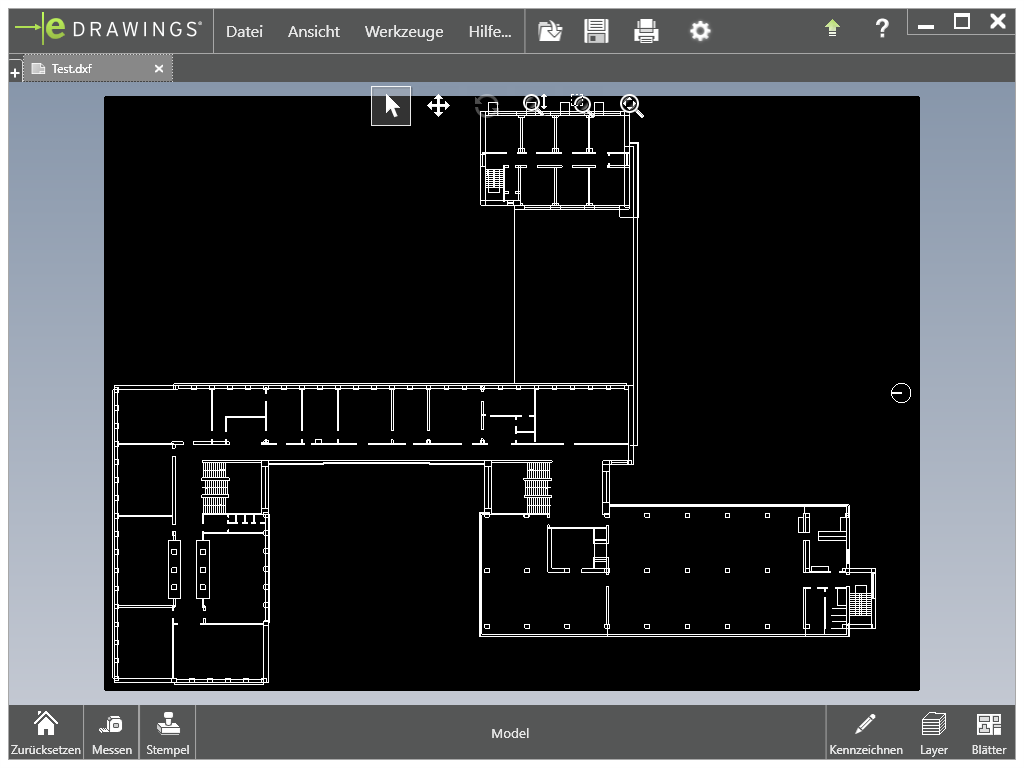
\includegraphics[width=0.5\textwidth]{res/edrawings-viewer.png}
    \caption{Screenshot des Programms \textit{eDrawings Viewer}.}
    \label{fig:edrawings-viewer}
\end{figure}

\subsubsection{ABViewer}
\label{subsubsec:abviewer}

Auch die Software \textit{ABViewer} kann zur Anzeige von CAD-Dateien - nach lokaler Installation - verwendet werden~\cite{ABViewer}.
Das Aussehen der Anwendung zum aktuellen Zeitpunkt ist im Bild~\ref{fig:abviewer} dokumentiert.
Wir finden erneut die klassischen Elemente, wie auch bei den bereits betrachteten Programmen: Verschieben und Zoomen mit der Maus (Pan and Zoom) sowie Messungen und Markierungen.

\begin{figure}
    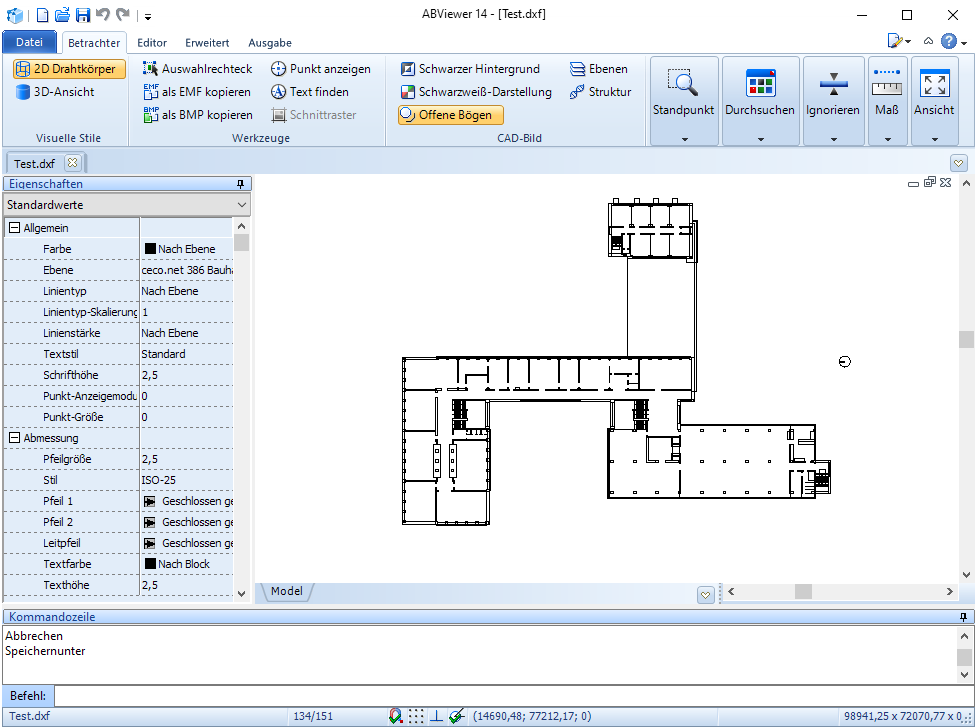
\includegraphics[width=0.5\textwidth]{res/abviewer.png}
    \caption{Screenshot des Programms \textit{ABViewer}.}
    \label{fig:abviewer}
\end{figure}

\subsubsection{DWG FastView}
\label{subsubsec:dwg-fastview}

Als letzte alternative Software betrachten wir das Programm \textit{DWG FastView}.
Das Produkt soll speziell zum Betrachten von CAD-Dateiformaten verwendet werden und ist in drei verschiedenen Ausführungen erhältlich: Online, für den Desktop und Mobilgeräte~\cite{DWGFastView}.

Die in Screenshot~\ref{fig:dwg-fastview-online} dargestellte Online-Version der Anwendung zeigt einen eher minimalistischen Viewer.
Lediglich die Navigation durch den geöffneten Beispielgebäudeplan ist möglich.
Weiterführende Merkmale, wie Messungen vorzunehmen oder Markierungen anzubringen, sind jedoch auch hier möglich; Allerdings nur unter Windows und auf Mobilgeräten in der kostenpflichtigen Premium-Version~\cite{DWGFastViewPremium}.

Ein Screenshot der Windows-Version ist in Abbildung~\ref{fig:dwg-fastview-windows} zu sehen.
Wie bereits erwähnt werden dort weiterführende Funktionen angeboten, die nicht in der minimalistischen Webapplikation zur Verfügung stehen.

\begin{figure}
    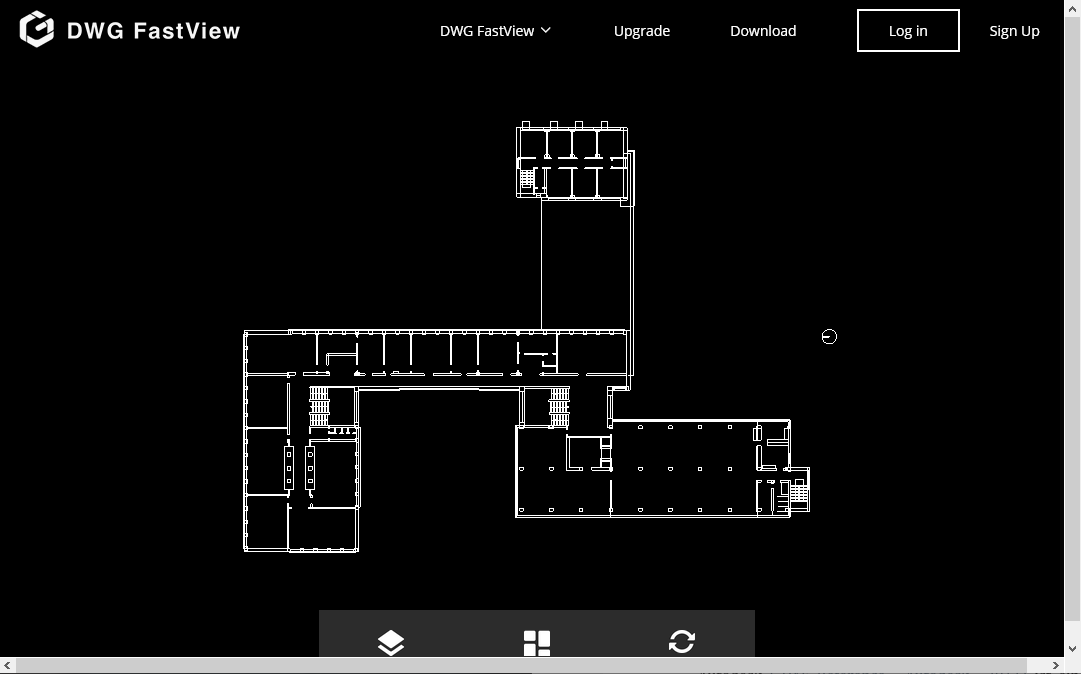
\includegraphics[width=0.5\textwidth]{res/dwg-fastview-online.png}
    \caption{Screenshot der Online-Version von \textit{DWG FastView}.}
    \label{fig:dwg-fastview-online}
\end{figure}

\begin{figure}
    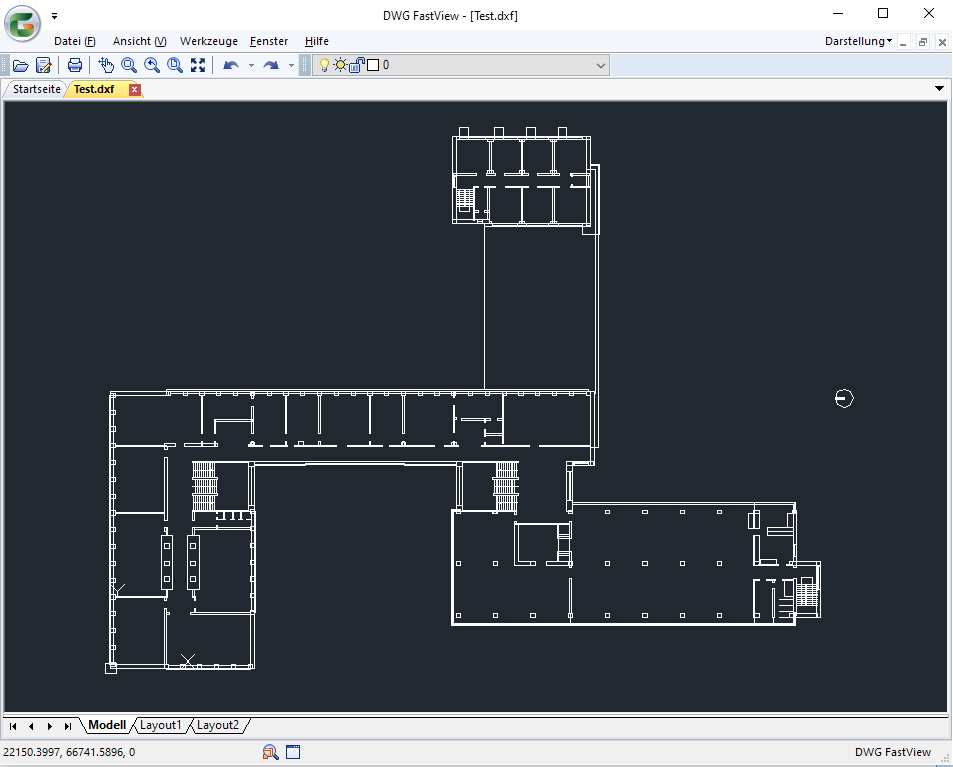
\includegraphics[width=0.5\textwidth]{res/dwg-fastview.png}
    \caption{Screenshot der Windows-Version von \textit{DWG FastView}.}
    \label{fig:dwg-fastview-windows}
\end{figure}
